%%%%%%%%%%%%%%%%%%%%%%%%%%%%%%%%%%%%%%%%%%%%%%%%%%%%%%%%%%%%%%%%%%%%%

%%%%%%%%%%%%%%%%%%%%%%%%%%%%%%%%%%%%%%%%%%%%%%%%%%%%%%%%%%%%%%%%%%%%%

\documentclass[11pt,a4paper,titlepage]{article}
\usepackage[utf8]{inputenc} 
\usepackage[english,icelandic]{babel}
\usepackage{t1enc}
\usepackage{hyperref}
\usepackage{amsmath}
\usepackage{amsfonts}
\usepackage{amssymb}
\usepackage{mdwlist} 
\usepackage{graphicx}
\usepackage{mcode}
  \parindent 0pt
  \lstset{language=matlab}
  \lstset{inputencoding=latin1}

%% Til a� breyta st�r� og sta�setningu textans � s��unni
% \voffset=-1.0in
% \hoffset=-0.3in
% \textwidth=6in
% \textheight=10.2in


% Eigin skipanir
\newcommand{\R}{{\Bbb R}}  

\title{T�luleg greining (ST�405G vor 2015)\\
Heimaverkefni I}
\date{\today}
\author{Gunna J�nsd�ttir og J�n Gunnuson}

\begin{document}


\section{Varmajafnvægi}
% Undirkafli
\subsection{}
Skrifa \verb|matlab|-forrit sem finnur nálgunarlausn á Sturm-Liouville-verkefninu (1.1) með Galerkin-aðferð og þúfugrunnföllum, þar sem gert er ráð fyrir að $p$ megi vera ósamfellt og að hægri hliðin megi innnihalda punktuppsprettu.

\textbf{Lausn:} 
Forritið er svona útlítandi \begin{verbatim}
function c=Galerkinadferd(p,q,f,x,alpha,beta,gamma,r,Q)

N=length(x);
h=x(2:N)-x(1:N-1);
m=(x(2:N)+x(1:N-1))/2;
pm=p(m);
qm=q(m);
fx=f(x);

A=zeros(N,3);
b=zeros(N,1);

A(2:N-1,2) = pm(1:N-2)./h(1:N-2)+pm(2:N-1)./h(2:N-1)+(h(1:N-2).*qm(1:N-2)+h(2:N-1).*qm(2:N-1))/3;
A(2:N,1) = -pm(1:N-1)./h(1:N-1)+h(1:N-1).*qm(1:N-1)/6;
A(1:N-1,3) = A(2:N,1);
b(2:N-1) = (h(1:N-2).*(fx(1:N-2)+2*fx(2:N-1))+h(2:N-1).*(2*fx(2:N-1)+fx(3:N)))/6;

if beta(1) == 0
    A(1,2) = alpha(1);
    A(1,3) = 0;
    b(1) = gamma(1);
else
    A(1,2) = pm(1)/h(1)+h(1)*qm(1)/3+p(x(1))*alpha(1)/beta(1);
    b(1) = h(1)*(2*fx(1)+fx(2))/6+p(x(1))*gamma(1)/beta(1);
end

if beta(2) == 0
    A(N,1) = 0;
    A(N,2) = alpha(2);
    b(n) = gamma(2);
else
    A(N,2) = pm(N-1)/h(N-1)+h(N-1)*(qm(N-1)/3)+(p(x(N))*(alpha(2)/beta(2)));
    b(N) = h(N-1)*(fx(N-1)+2*fx(N))/6+p(x(N))*(gamma(2)/beta(2));
end

if ~isempty(r)
m=length(r);
for j=1:m
    i=max(find(x<=r(j)));
    b(i-1)=b(i-1)+Q(j)*(1-(r(j)-x(i-1))/(x(i)-x(i-1)));
    b(i) = b(i)+Q(j)*(r(j)-x(i-1))/(x(i)-x(i-1));
end
end

c=tridiagonal_solve(A,b);
\end{verbatim}

\subsection{}
Rökstyðjið að aðferð Galerkins virki með ósamfellt $p$ eins og lýst er hér að framan. Það eina sem þarf að gera að sýna að hlutheildunin sem liggur t il grundvallar aðferðinni virki í þessu tilfelli þegar $p$ er ósamfellt eins og lýst er hér að framan. 

\textbf{Lausn:} 

\subsection{}
Gerið grein fyrir því hvernig punktuppspretturnar eru meðhöndlaðar í forritinu. Sýnið með einni keyrslu hvaða áhrif það hefur á lausn ef punktuppsprettu er bætt við hægri hliðina. 

\textbf{Lausn:} 

\subsection{}
Finnið sjálf heppilegt sýnidæmi til þess að prófa hvort forritið virki réttt. Kannið hvort skekkjan í nálguninni er $O(h^2)$, þar sem $h$ táknar billengd í jafnri skiptingu með því að prófa forritið í sýnidæminu með fjölda bila $N$=2,4,8....

\textbf{Lausn:} 
Heppilegt sýnidæmi sem við fundum í heimadæmum 8.1. Byrjum á því að skilgreina breyturnar. 
\begin{verbatim}
p = @(x) x;
q = @(x) 1./x;
f = @(x) -2 + 0.*x;
u=@(x) x.*log(x)-x;
x = [1:1/3:2];
alpha=[0,1];
beta = [-1,-2];
gamma=[0,-2];
r=2;
Q=0;
\end{verbatim}
Köllum svo á fallið. 
\begin{verbatim}

>> galerkinadferd_2(@(x)x,@(x)(1./x),@(x)-2+0.*x,[1:1/3:2],[0,1],[-1,-2],[0,-2],2,0)

ans =

   -0.9977
   -0.9424
   -0.8039
   -0.5987
\end{verbatim}
 Plottum svo upp. 
 \begin{verbatim}
 >> plot(linspace(1,2,4),ans)
 >> hold on
 >> plot(linspace(1,2,100),u(linspace(1,2,100)),'r')
 \end{verbatim}
 
 Fáum þá út fallið og nálgunarfallið. 
 
  \begin{figure}[h!]
      \centering
      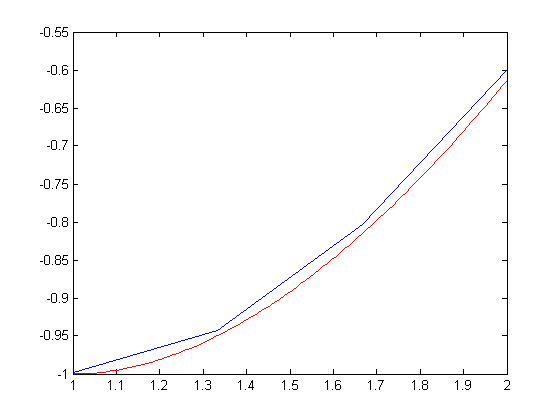
\includegraphics[width=0.9\textwidth]{nalgun1_4.png}
      \caption{Contour-mynd af Söðulmynd}
      \label{fig:awesome_image1}
  \end{figure}
\section{Straujárnið hennar Mömmu}
\subsection{}
Skrifið \verb|matlab|-forrit sem notar forritið ykkar \verb|Galerkinadferd| úr síðasta lið til þess að finna nálgun á lausn þessa verkefnis. Notið fjögurra punkta skiptingu  $x_{0}=a, x_{1}=s, x_{2}=r$ og $x_{3}=b$.  Framkvæmið fastapunktsítrekunina þar til endurbítin í ítrekuninni er innan við 1\%.  MArkmiðið er að þið prófið ykkur áfram með að stilla gildið á Q þannig að út komi hitastigið $u(b)\approx 200°C$. (Hámarksafllið í venulegu straujárni er 1200-1500W.) Þegar þetta gildi á Q er fundið eigði þi ða teikna upp hitastigið sem fall af $x$. 

\textbf{Lausn:}
\begin{verbatim}

\end{verbatim}


\subsection{}


\textbf{Lausn:}

\subsection{}
Útskýrið hvað gerist ef tekin er fínni skiptinn

\textbf{Lausn:}


\section{Dirichlet verkefnið á rétthyrningi}

\subsection{}

Útfæra Dirichletverkfni í  \verb|matlab|. 

\textbf{Lausn:}
\begin{verbatim}
function [W,A,RHS]=Dirichletverkefni(a,b,c,d,p,q,f,gamma,P,Q,R,U,h)
%Author: Andri Freyr Thorgeirsson, Erna Gudrun Thorsteinsdottir og
%        Rikhardur Thor Rognvaldsson

% Breytur

% Setja upp reikninetid
M=(b-a)/h+1;               % Fjoldi hnitpunkta i x att
N=(d-c)/h+1;            % Fjoldi hnitpunkta i y att
% Skilgreinum staerd fylkis og haegri handar
A=zeros(M*N,M*N);       % Fylkid okkar er jafn stort og fjoldi punkta
RHS=zeros(M*N,1);       % Haegri hlid hefur somu staerd og fylkid en er vigur
ki = 1;                 % Dummy breyta fyrir visun í Rs
kj = 1;                 % Dummy breyta fyrir vísun í Qs
%Setjum gildi i fylki og haegri hlid
%Byrjum a því að finna nalgunargildi á R og Q
x_vigur = linspace(a,b,M);
y_vigur = linspace(c,d,N);
r_hnit=NaN;
p_hnit=NaN;
if ~isempty(R)
    r_hnit = zeros(length(R(1,:)),length(R(:,1)));
    for i = 1:length(R(:,1))
        r_hnit(i,1) = min(find(x_vigur>=R(i,1)));
        r_hnit(i,2) = min(find(y_vigur>=R(i,2)));
    end
end
if ~isempty(P)
    
    p_hnit = zeros(length(P(1,:)),length(P(:,1)));
    for j = 1:length(R(:,1))
        p_hnit(j,1) = min(find(x_vigur>=P(j,1)));
        p_hnit(j,2) = min(find(y_vigur>=P(j,2)));
    end
end



for n=1:N
    for m=1:M
        
        % Vid kjosum ad rada T_m,n thar sem fyrst er n=1 og m haekkar fra 1 til M,
        % Thvi naest haekkum vid n i 2 og haekkum m fra 1 til M, haekkum tha n i 3 og
        % haekkum m fra 1 til M og svo framvegis thar til m is jafnt M
        
        s=m+M*(n-1);               % Numer linu fylkis sem samsvarar m,n
        s_m_plus1=m+1+M*(n-1);     % Numer linu fylkis sem samsvarar m+1,n
        s_m_minus1=m-1+M*(n-1);    % Numer linu fylkis sem samsvarar m-1,n
        s_n_plus1=m+M*(n+1-1);     % Numer linu fylkis sem samsvarar m,n+1
        s_n_minus1=m+M*(n-1-1);    % Numer linu fylkis sem samsvarar m,n-1
        x = a+(m-1)*h;
        y = c+(n-1)*h;
        x_half = a+(m-1)*(h/2);
        y_half = c+(n-1)*(h/2);
        % Viðbót 2 - fast gildi í ákveðnum punkti
        
        % Jaðarskilyrði - u = gamma
        % Skilyrdi: (n==1) -> Viljum skoda nedstu linuna kassans
        % Skilyrdi: (n==N) -> Viljum skoda efstu linuna kassans
        % Skilyrdi: (m==1) -> Viljum skoda vinstri hlid kassans
        % Skilyrdi: (m==M) -> Viljum skoda haegri hlid kassans
        if  (m==1) || (M==m) || (n==1) || (N==n)
            A(s,s) = 1;
            RHS(s) = gamma(x,y);
            fprintf('Jadarpunktur n=%.0f , m = %.0f\n',n,m)
        end
        
        % Innri hnutpunktar kassans - jafna 22.3
        % Skilyrdi: (n>1)  -> Viljum ekki skoda nedstu linuna
        % Skilyrdi: (m>n) -> Viljum lenda haegra meginn vid vinstri
        %                    hlidarlinu thrihyrningsins
        % Skilyrdi: (m<M-n+1) -> Viljum lenda vinstra meginn vid haegri
        %                        hlidarlinu thrihyrningsins
        % Skilyrdi: (n<N) -> Viljum ekki lenda i topppunktinum.
        if (n>1) && (m>1) && (m<M) && (n<N)
            A(s,s) = ((p(x_half+h,y)+p(x_half-h,y)+p(x,y_half-h)+p(x,y_half+h))/h^2)+q(x,y);
            A(s,s_m_plus1) = -p(x_half+h,y)/h^2;   %p_j,r
            A(s,s_m_minus1) = -p(x_half-h,y)/h^2;  %p_j,l
            A(s,s_n_plus1) = -p(x,y_half+h)/h^2;   %p_j,t
            A(s,s_n_minus1) = -p(x,y_half-h)/h^2;  %p_j,s
            RHS(s) = f(x,y);
            fprintf('Innripunktur n=%.0f , m = %.0f\n',n,m)
            if ~isnan(p_hnit)
                if m == p_hnit(kj,1) && p_hnit(kj,2) == n && kj<=length(P(:,1))
                    RHS(s) = f(x,y)+sum(Q(kj)/h^2);
                    kj=kj+1;
                    fprintf('Sérstöðupunktur - Punktuppspretta x=%.2f , y = %.2f , n=%.0f , m = %.0f\n',x,y,n,m)
                end
            end
        end
        if  ki<=length(R(:,1))
            if m == r_hnit(ki,1) && r_hnit(ki,2) == n 
                A(s,:) = 0;
                A(s,s) = 1;
                RHS(s) = U(ki);
                ki = ki+1;
                fprintf('Sérstöðupunktur - FAST GILDI x=%.2f , y = %.2f , n=%.2f , m = %.0f\n',x,y,n,m)
                disp(A(s,:))
            end
        end
    end
end
%Finnum lausn
A_sparse=sparse(A);
W_list=A_sparse\RHS;   % Thetta er vigur med hitastigum rodudum eins og vid til-
% greindum ad ofan
T_grid=zeros(N,M);
for n=1:N
    for m=1:M
        s=m+M*(n-1);   % Numer linu fylkis sem samsvarar m,n
        T_grid(n,m) = W_list(s); % Setjum inn gildi sem samsvarar
        % gildi fyrir thrihyrninginn okkar.
    end
end
W=T_grid;

\end{verbatim}
\subsection{}
Útskýrið hvers vegna uppsprettuliðirnnir eru meðhöndlaðir með því að setja $b_{j} = f(x_{j},y_{k})+h^{-2}$ ef $(x_{j},y_{j})$ er sá punktur netsins sem næstur er $P_s$.  
\textbf{Lausn:}

\subsection{}
Þið þurfið að sannfæra ykkur um forritið reikni rétt.  Tökum t.d. fallið $u(x,y)=x^2-y^2$ veljið D=[-1,1]x[-1,1], og $\gamma(x,y)=x^2-y^2$ á öllum jaðrinum, þá eigið þið að fá nálgunarfall sem er nánast eins og rétta lausnin.
\textbf{Lausn:}
byrjum á því að skilgreina breyturnar okkar. 
\begin{verbatim}
a=-1;
b=1;
c=-1;
d=1;
gamma= @(x,y) x.^2-y.^2;
p=@(x,y) 1;
q=@(x,y) 0;
f=@(x,y) 0;
h= 0.1;
\end{verbatim}

Köllum svo á fallið:
\begin{verbatim}
>> [W,A,RHS]=Dirichletverkefni(a,b,c,d,p,q,f,gamma,[1,1],[0],[1,0],[1],0.1)
>> surf(linspace(a,b,length(W(:,1))),linspace(c,d,length(W(1,:))),W'); 
\end{verbatim}
 \begin{figure}[h!]
     \centering
     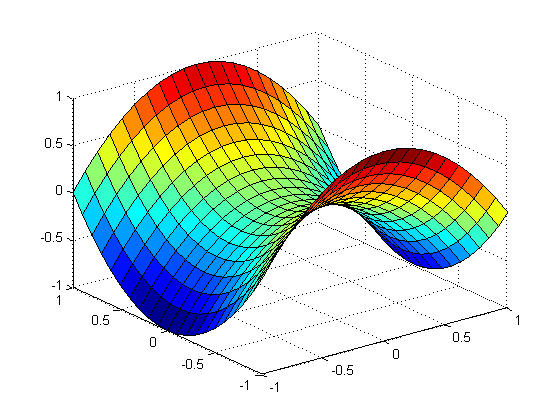
\includegraphics[width=0.9\textwidth]{sodulmynd1.png}
     \caption{Söðulmynd}
     \label{fig:awesome_image1}
 \end{figure}
 \newpage
þessi liður gefur okkur svo contour af fallinu. 
\begin{verbatim}
>> contour(linspace(a,b,length(W(:,1))),linspace(c,d,length(W(1,:))),W');
\end{verbatim}
 \begin{figure}[h!]
     \centering
     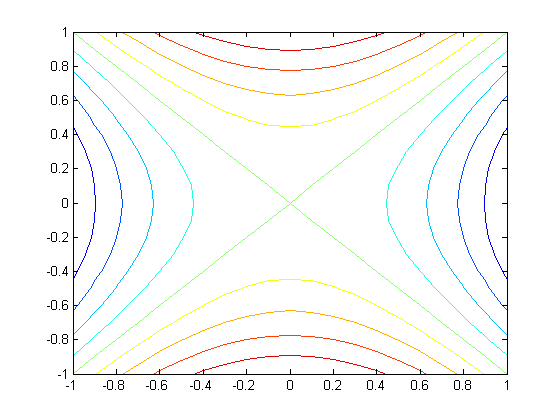
\includegraphics[width=0.9\textwidth]{sodulmynd_contour.png}
     \caption{Contour-mynd af Söðulmynd}
     \label{fig:awesome_image1}
 \end{figure}
\newpage


\subsection{}
Notið forritið ykkar til að þess að taka svæðið á D]-1,1]x[-1,1[, og reikna út og teikna upp lausinina á 




$
\left\{\begin{matrix}
$$\nabla^2u=0
\\ 
\alpha=1, \beta=0, \gamma(x,y)$$
\end{matrix}\right.
$
= 
$
 \left\{\begin{matrix}
  5max
 \begin{Bmatrix}
 $$cos(\pi y),0\end{Bmatrix}
 , x=\pm 1,\
 \\5max
 \begin{Bmatrix}
 cos(\pi y),0
 \end{Bmatrix}, y= \pm 1. 
 $$
 
 \end{matrix}\right.
 $
 
 
 Setjið teikningu af grafi lausnarinnar í skýrsluna. 
 
 \textbf{Lausn:}
 
 Byrjum á því að skilgreina breyturnar.
 \begin{verbatim}
 a=-1;
 b=1;
 c=-1;
 d=1;
 gamma= @(x,y) x.^2-y.^2;
 p=@(x,y) 1;
 q=@(x,y) 0;
 f=@(x,y) 0;
 h= 0.1;
 \end{verbatim}
 Svo köllum við á fallið:
 \begin{verbatim}
 >>[W,A,RHS]=Dirichletverkefni(a,b,c,d,p,q,f,gamma,[],[],[],[],0.1)
 >> surf(linspace(a,b,length(W(:,1))),linspace(c,d,length(W(1,:))),W');
 \end{verbatim}
Sjáum að myndin líkist kirkjunni í Kópavogi.
  \begin{figure}[h!]
      \centering
      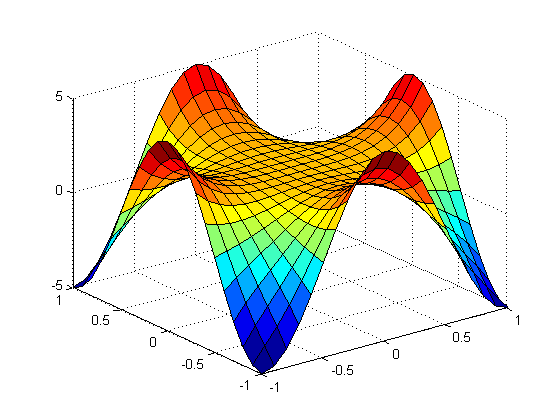
\includegraphics[width=0.9\textwidth]{gudshusid.png}
      \caption{Guðshúsið í Kópavogi}
      \label{fig:awesome_image1}
  \end{figure} 
  
  
 Köllum svo aftur á fallið til að fá contour-mynd.
 \begin{verbatim}
 >> contour(linspace(a,b,length(W(:,1))),linspace(c,d,length(W(1,:))),W');
 \end{verbatim}
 
 Fáum þá út myndina.
 
 \begin{figure}[h!]
       \centering
       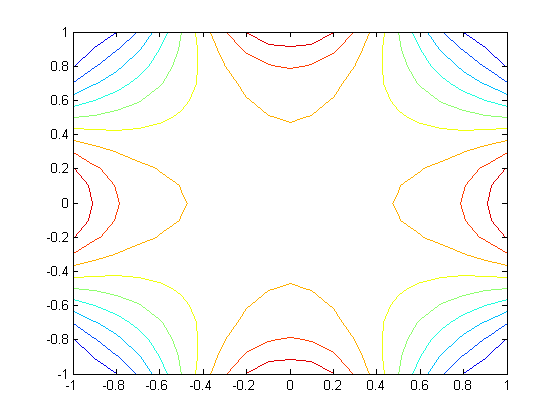
\includegraphics[width=0.9\textwidth]{gudshusid_contour.png}
       \caption{Countour-mynd af Guðshúsinu í Kópavogi}
       \label{fig:awesome_image1}
   \end{figure}
   
\newpage
 
 \subsection{}
 Líkið eftir Hróarskeldutjaldinu. Útskýrið hvaða formúlur þið notað og setjið myndí skýrsluna. 
 
 \textbf{Lausn:}
 
 Byrjum á því að skilgreina eftirfarandi breytur:
 \begin{verbatim}
 a=-2;
 b=2;
 c=-0.5;
 d=2;
 gamma=@(x,y) hroarskelda_gamma(x,y);
 p = @(x,y) 1+0.*x+0.*y;
 q = @(x,y) 0+0.*x+0.*y;
 f = @(x,y) 0+0.*x+0.*y;
 h=0.1;
 \end{verbatim}
 Aukaforritið   \verb|hroarskelda_gamma.m| er hægt að finna í viðauka hér að neðan.  Við köllum svona á forritið til að fá eftirfarandi mynd:
 \begin{verbatim}
 >>[W,A,RHS]=Dirichletverkefni(a,b,c,d,p,q,f,gamma,[],[0],[0,0;-0.9,1;0.9,1],[1,1,1],0.1);
 >> surf(linspace(a,b,length(W(:,1))),linspace(c,d,length(W(1,:))),W');
 
 \end{verbatim}
 Sjáum hér að ofan hvað  \verb|a,b,c,d,p,q,f,gamma| er skilgreint sem. 
 
 Við völdum að þar sem punktuppspretturnar myndu byrja væru hnitin  \verb|[0,0],[-0.9,1],[0.9,1]|  síðan hvað "magnitude-ið" væri á þessum punktuppsprettum en allar höfðu þær styrkinn 1. Út kom þá eftirfarandi myndir. 
 
 \begin{figure}[h!]
     \centering
     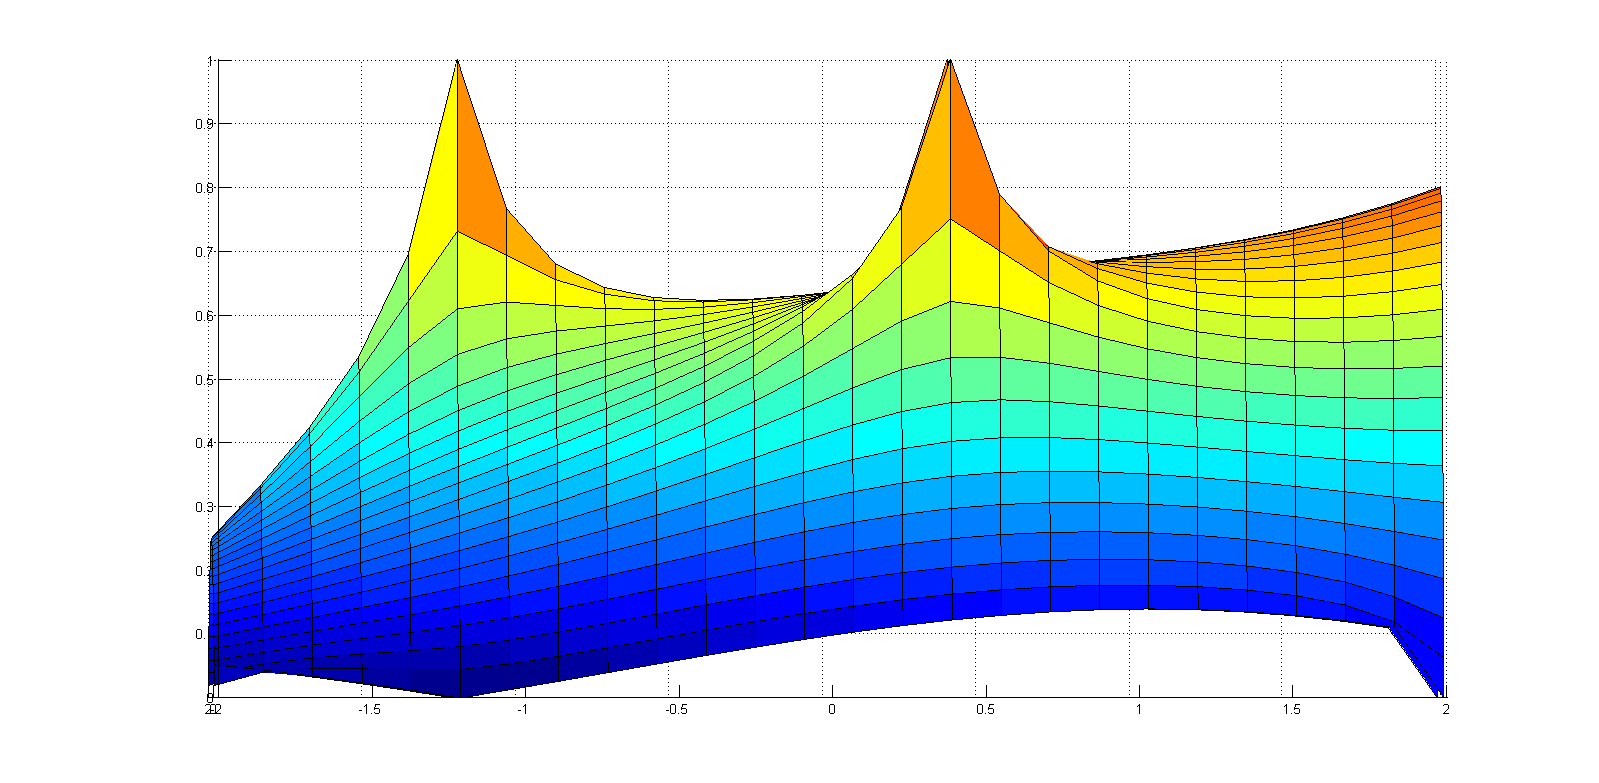
\includegraphics[width=0.9\textwidth]{hroarskelda_hlid.png}
     \caption{Hróarskeldutjaldið á hlið}
     \label{fig:awesome_image1}
 \end{figure}
 
 \begin{figure}[h!]
     \centering
     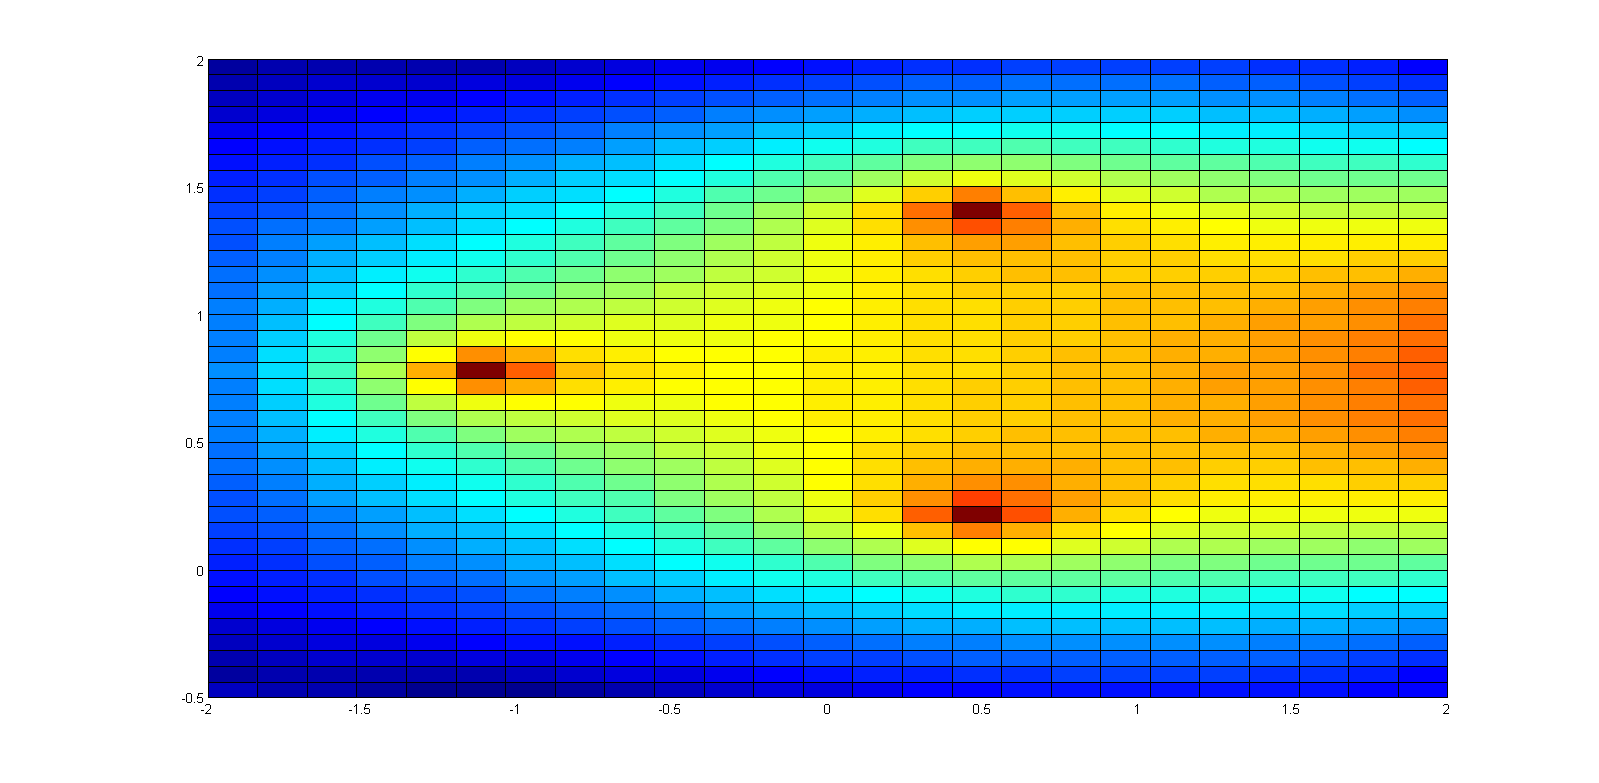
\includegraphics[width=0.9\textwidth]{hroarskelda_top.png}
     \caption{Hróarskeldutjaldið ofan frá }
     \label{fig:awesome_image1}
 \end{figure}
 
  \begin{figure}[h!]
      \centering
      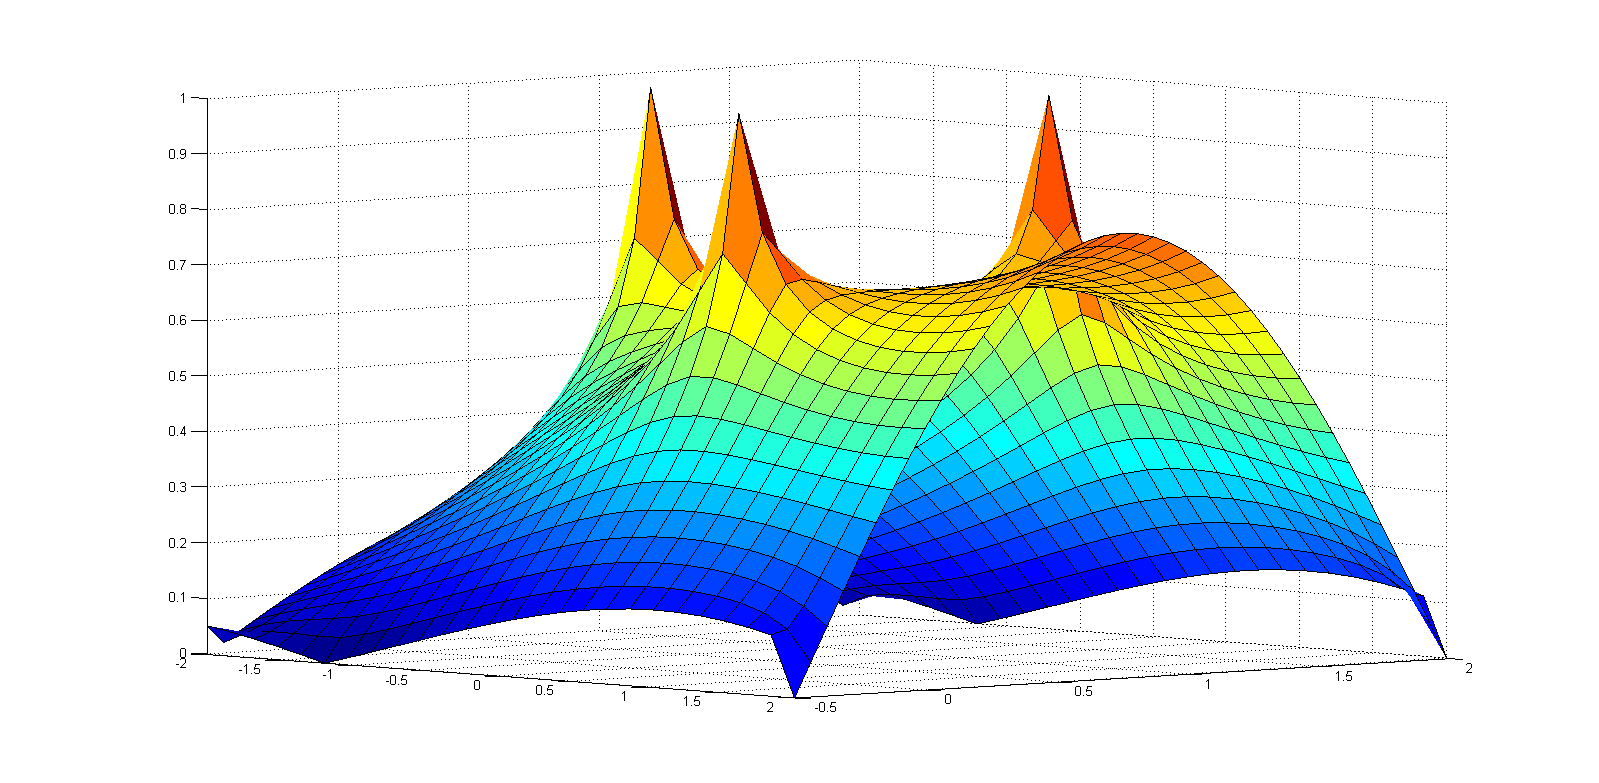
\includegraphics[width=0.9\textwidth]{hroarskelda_party.png}
      \caption{Hróarskeldutjaldið í allri sinni dýrð}
      \label{fig:awesome_image1}
  \end{figure}
  \newpage
  
  
 \subsection{}
 Hannið nýtt tjald til þess að setja upp við Arnarhól á menningarnótt í Reykjavík. Útskýrið hönnunina og setjið mynd í skýrsluna.
 
 \textbf{Lausn:}
 
 
 
 \section{Lágmarksfletir}
 
 \subsection{}
u\left ( x,y \right)  \sqrt{\cosh (x)^{2}-y^{2}}  uppfyllir hlutafleiðujöfnuna fyrir lágmarksflöt. Notið það á rétthyrningnum D = [-1,1] * [-1,1] til þess að kanna hvort forritið reiknar rétt
 
 \subsection{}
 Gerið grein fyrir stærð netsins sem þið notið, hvaða þolmörk þið notið til þess að stöðva ítrekunina og hversu langan tíma keyrslan tók á tölvunni ykkar.
 
 \subsection{}
 Berið saman á mynd hver munurinn er á því sem fékkst út í upphafsskrefinu og lokaskrefinu. Þetta má einfaldlega gera með því að teikna upp mismuninn.
 
 \subsection{}
 Keyrið forritið með dæmið ykkar um Hróarskeldutjaldið eða Arnarhólstjaldið. Hver er munurinná lausninni á jöfnunni fyrir lágmarksflöt miðað við graf lausnarinnar á Laplace-jöfnu meðsömu jaðarskilyrðum. Setjið fallega mynd á forsíðuna
 
 
\newpage
\begin{flushright}
 \today
\end{flushright}
\end{document}
